% -*- mode: latex; mode: visual-line; fill-column: 9999; coding: utf-8 -*-

\section{Computational Experiments}
\label{sec:experiments}

We had previously measured the performance of the MPI-parallelized RMSD analysis task on two different HPC resources (\emph{SDSC Comet} and \emph{TACC Stampede}) and had found that it only scaled well up to a single node due to high variance in the runtime of the MPI ranks, similar to the straggler phenomenon observed in big-data analytics \cite{Khoshlessan:2017ab}.
However, the ultimate cause for this high variance could not be ascertained.
We therefore performed more measurements with more detailed timing information (see section \ref{sec:methods}) on \emph{SDSC Comet} (described in this section) and two other supercomputers (summarized in section \ref{sec:clusters}) in order to better understand the origin of the stragglers and find solutions to overcome them. 

\subsection{RMSD Benchmark}
\label{sec:RMSD}

We measured strong scaling for the RMSD analysis task (Algorithm \ref{alg:RMSD}) with the 2,512,200 frame test trajectory (section \ref{sec:data}) on 1 to 72 cores (one to three nodes) of \emph{SDSC Comet} (Figures~\ref{fig:MPIscaling} and \ref{fig:MPIspeedup}). 
We observed poor strong scaling performance beyond a single node (24 cores), comparable to our previous results \cite{Khoshlessan:2017ab}.
A more detailed analysis showed that the RMSD computation, and to a lesser degree the read I/O, considered on their own, scaled well beyond 50 cores (yellow and blue lines in Figure~\ref{fig:ScalingComputeIO}). 
But communication (sending results back to MPI rank 0 with \texttt{MPI\_Gather()}; red line in Figure~\ref{fig:ScalingComputeIO}) and the initial file opening (loading the system information into the \texttt{MDAnalysis.Universe} data structure from a shared ``topology'' file and opening the shared trajectory file; gray line in Figure~\ref{fig:ScalingComputeIO}) started to dominate beyond 50 cores.
Communication cost and initial time for opening the trajectory were distributed unevenly across MPI ranks, as shown in Figure~\ref{fig:MPIranks}. 
The ranks that took much longer to complete than the typical execution time of the other ranks were the stragglers that hurt performance.

\begin{figure}[!htb]
  \centering
  \begin{subfigure}{.49\textwidth}
    \includegraphics[width=\linewidth]{figures/main-RMSD-t_total.pdf}
    \captionsetup{format=hang}
    \caption{Scaling total (five repeats)}
    \label{fig:MPIscaling}
  \end{subfigure}
  \hfill
  \begin{subfigure}{.49\textwidth}
    \includegraphics[width=\linewidth]{figures/main-RMSD-speed_up.pdf}
    \captionsetup{format=hang}
    \caption{Speed-up (five repeats)}
    \label{fig:MPIspeedup}
  \end{subfigure}
  \bigskip

  \begin{subfigure}{.49\textwidth}
    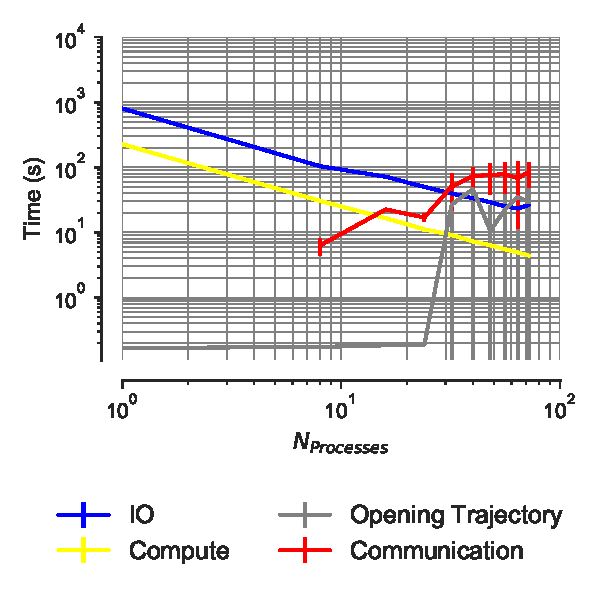
\includegraphics[width=\linewidth]{figures/main-RMSD-time_comp_IO_comparison.pdf}
    \captionsetup{format=hang}
    \caption{Scaling for different components (five repeats)}
    \label{fig:ScalingComputeIO}
  \end{subfigure}
  \hfill
  \begin{subfigure} {.5\textwidth}
    \includegraphics[width=\linewidth]{figures/main-RMSD-BarPlot-rank-comparison_72_5.pdf}
    \captionsetup{format=hang}
    \caption{Time comparison on different parts of the calculations per MPI rank (example)}
    \label{fig:MPIranks}
  \end{subfigure}
  \caption{Performance of the RMSD task parallelized with MPI on \emph{SDSC Comet}.
    Results were communicated back to rank 0.
    Five independent repeats were performed to collect statistics.
    (a-c) The error bars show standard deviation with respect to the mean.
    In serial, there is no communication and no data points are shown for $N=1$ in (c).
    (d) Compute \tcomp, read I/O \tIO, communication \tcomm, ending the for loop $t_{\text{end\_loop}}$, opening the trajectory $t_{\text{opening\_trajectory}}$, and overheads $t_{\text{overhead1}}$, $t_{\text{overhead2}}$ per MPI rank; see Table \ref{tab:notation} for definitions.
    These are data from one run of the five repeats.
    MPI ranks 0, 12--27 and 29--72 are stragglers.
  }
  \label{fig:MPIwithIO}
\end{figure}

We qualitatively denoted by \emph{straggler} any MPI rank that took at least about twice as long as the group of ranks that finished fastest, roughly following the original description of a straggler as a task that took an ``unusually long time to complete'' \cite{Dean2008}.
The fast-finishing ranks were generally clearly distinguishable in the per-rank timings such as in Figures~\ref{fig:MPIranks} and \ref{fig:MPIranks-Bridges}.
Such a qualitative definition of stragglers was sufficient for our purpose to identify scalability bottlenecks, as shown in the following discussion.

\subsubsection*{Identification of Scalability Bottlenecks}

In the example shown in Figure~\ref{fig:MPIranks}, 62 ranks out of 72 took about 60~s (the stragglers) whereas the remaining ranks only took about 20~s.
In other instances, far fewer ranks were stragglers, as shown, for example, in Figure~\ref{fig:MPIranks-Bridges}.
The detailed breakdown of the time spent on each rank (Figure~\ref{fig:MPIranks}) showed that the computation, \tcomp, was relatively constant across ranks. 
The time spent on reading data from the shared trajectory file on the Lustre file system into memory, \tIO, showed variability across different ranks. 
The stragglers, however, appeared to be defined by occasionally much larger \emph{communication} times, \tcomm (line 16 in Algorithm~\ref{alg:RMSD}), which were on the order of 30~s, and by larger times to initially open the trajectory (line 2 in Algorithm~\ref{alg:RMSD}).
\tcomm varied across different ranks and was barely measurable for a few of them.
Although the data in Figure~\ref{fig:MPIranks} represented one run and in other instances different number of ranks were stragglers, the averages over all ranks in five independent repeats (Figure~\ref{fig:ScalingComputeIO}) showed that increased \tcomm were generally the reason for large variations in the run time for each rank.
This initial analysis indicated that communication was a major issue that prevented good scaling beyond a single node but the problems related to file I/O also played an important role in limiting scaling performance.


\subsubsection*{Influence of Hardware}
We ran the same benchmarks on multiple HPC systems that were equipped with a Lustre parallel file system [XSEDE's \emph{PSC Bridges} (Fig.~\ref{fig:MPIwithIO-Bridges}) and \emph{LSU SuperMIC} (Fig.~\ref{fig:MPIwithIO-SuperMIC})], and observed the occurrence of stragglers, in a manner very similar to the results described for \emph{SDSC Comet}.
There was no clear pattern in which certain MPI ranks would always be a straggler, and neither could we trace stragglers to specific cores or nodes.
Therefore, the phenomenon of stragglers in the RMSD case was reproducible on different clusters and thus appeared to be independent from the underlying hardware.

\subsection{Effect of Compute to I/O Ratio on Performance}
\label{sec:bound}

The results in section~\ref{sec:RMSD} indicated opening the trajectory, communication, and read I/O to be important factors that appeared to correlate with stragglers. 
In order to better characterize the RMSD task, we computed the ratio between the time to complete the computation and the time spent on I/O per frame.
The average values were $\overline{\tcomp^{\text{frame}}} = 0.09\ \text{ms}$, $\overline{t_{\text{IO}}^{\text{frame}}} = 0.3\ \text{ms}$, resulting in a compute-to-I/O ratio $\RcompIO \approx 0.3$ (Eq.~\ref{eq:Compute-IO}).
Because $\RcompIO \ll 1$, the RMSD analysis task was characterized as I/O bound.

As we were not able to achieve good scaling beyond a single node, we hypothesized that decreasing the I/O load relative to the compute load would interleave read I/O with longer periods of computation, thus reducing the impact of I/O contention and the impact of stragglers.
We therefore set out to measure compute bound tasks, i.e.\ ones with $\RcompIO \gg 1$.
To measure the effect of the $\RcompIO$ ratio on performance but leaving other parameters the same, we artificially increased the computational load by repeating the same RMSD calculation (line 10, algorithm \ref{alg:RMSD}) 40, 70 and 100 times in a loop, resulting in forty-fold (``$40\times$''), seventy-fold (``$70\times$''), and one hundred-fold (``$100\times$'') load increases.

\subsubsection{Effect of Increased Compute Workload}

For an $X$-fold increase in workload, we expected the workload for the computation to scale with $X$ as $\tcomp(X) =  N_{\text{frames}}^{\text{total}} X \overline{\tcomp^{\text{frame}}}$ while the read I/O workload $\tIO(X) = N_{\text{frames}}^{\text{total}} \overline{\tIO^{\text{frame}}}$ (number of frames times the average time to read a frame) should remain independent of $X$.
Therefore, the ratio for any $X$ should be $\RcompIO(X) = \tcomp(X)/\tIO(X) = X \RcompIO(X=1)$, i.e.,  $\RcompIO$ should just linearly scale with the workload factor $X$.
The measured $\RcompIO$ ratios of 11, 19, 27 for the increased computational workloads agreed with this theoretical analysis, as shown in Table \ref{tab:load-ratio}.

\begin{table}[!htb]
\centering
\begin{tabular}{rrrrr}
  \toprule
  \bfseries\thead{Workload $X$} &  \bfseries\thead{$\tcomp$ (s)} &  \bfseries\thead{$\tIO$ (s)}
  & \multicolumn{2}{c}{\bfseries\thead{$\RcompIO$}}\\
  & & & \thead{measured} & \thead{theoretical}\\
  \midrule
    $1\times$   &   226 & 791 &  0.29 &   \\  
    $40\times$  &  8655 & 791 & 11   & 11\\    
    $70\times$  & 15148 & 791 & 19   & 20\\  
    $100\times$ & 21639 & 791 & 27   & 29\\  
  \bottomrule
\end{tabular}
\caption[Change in load-ratio with RMSD workload]{Change in $\RcompIO$ ratio with change in the RMSD workload $X$.
  The RMSD workload was artificially increased in order to examine the effect of compute to I/O ratio on the performance.
  The reported compute and I/O time were measured based on the serial version using one core.
  The theoretical $\RcompIO$ (see text) is provided for comparison.}
\label{tab:load-ratio}
\end{table}

\begin{figure}[!htb]
  \centering
  \begin{subfigure} {.3\textwidth}
    \includegraphics[width=\linewidth]{figures/Compute_to_IO_ratio_on_performance_2d_v17.pdf}
    \caption{Speed-Up}
    \label{fig:S1_tcomp_tIO_effect}
  \end{subfigure}
  \hfill
  \begin{subfigure}{.3\textwidth}
    \includegraphics[width=\linewidth]{figures/Compute_to_IO_ratio_on_performance_2d_2_v17.pdf}
    \caption{Speed-Up}
    \label{fig:S2_tcomp_tIO_effect}
  \end{subfigure}
  \hfill
  \begin{subfigure}{.3\textwidth}
    \includegraphics[width=\linewidth]{figures/Compute_to_IO_ratio_on_performance_2d_3_v17.pdf}
    \caption{Efficiency}
    \label{fig:E_tcomp_tIO_effect}
  \end{subfigure}
  \caption{Effect of $\RcompIO$ ratio on performance of the RMSD task on \emph{SDSC Comet}. We tested performance for $\RcompIO$ ratios of 0.3, 11, 19, 27, which correspond to $1\times$ RMSD, $40\times$ RMSD, $70\times$ RMSD, and $100\times$ RMSD respectively.
    (a) Effect of $\RcompIO$ on the speed-up.
    (b) Change in speed-up with respect to $\RcompIO$ for different processor counts.
    (c) Change in the efficiency with respect to $\RcompIO$ for different processor counts.}
  \label{fig:tcomp_tIO_effect}
\end{figure}

We performed the experiments with increased workload to measure the effect of the $\RcompIO$ ratio on performance (Figure~\ref{fig:tcomp_tIO_effect}).
The strong scaling performance as measured by the speed-up $S(N)$ improved with increasing $\RcompIO$ ratio (Figure \ref{fig:S1_tcomp_tIO_effect}).
The calculations consistently showed better scaling performance to larger numbers of cores for higher $\RcompIO$ ratios, e.g., $N=56$ cores for the $70\times$ RMSD task. 
The speed-up and efficiency approached their ideal value for each processor count with increasing $\RcompIO$ ratio (Figures \ref{fig:S2_tcomp_tIO_effect} and \ref{fig:E_tcomp_tIO_effect}).
Even for moderately compute-bound workloads, such as the $40\times$ and $70\times$ RMSD tasks, increasing the computational workload over I/O reduced the impact of stragglers even though they still contributed to large variations in timing across different ranks and thus irregular scaling.

We also investigated the influence of the ratio of compute to communication costs ($\Rcompcomm$, Eq.~\ref{eq:Compute-comm}) on performance in \ref{sec:tcomm}.
We found evidence to support the hypothesis that a larger ratio was beneficial, provided I/O costs could also be reduced.
However, read I/O ultimately seemed to be the key determinant for performance, as discussed in the next sections.


\subsubsection{Effect of Absence of Read I/O on Communication}

 \begin{figure}[!htb]
   \centering
   \begin{subfigure}{.35\textwidth}
     \includegraphics[width=\linewidth]{figures/speed_up-effect-of-IO.pdf}
     \caption{Speed up comparison}
     \label{fig:MPIspeedup-no-IO}
   \end{subfigure}
   \hfill
   \begin{subfigure}{.45\textwidth}
     \includegraphics[width=\linewidth]{figures/BarPlot-rank-comparison-no-IO.pdf}
     \captionsetup{format=hang}
     \caption{Time comparison on different parts of the calculations per MPI rank when I/O is removed}
     \label{fig:MPIranks-no-IO}
   \end{subfigure}
   \caption{Comparison of the performance of the RMSD task with I/O ($\RcompIO \approx 0.3$) and without I/O ($\RcompIO = +\infty$) on \emph{SDSC Comet}.
     Five repeats were performed to collect statistics.
     (a) Speed-up. The error bars show standard deviation with respect to the mean.
     (b) Compute \tcomp, read I/O $\tIO=0$, communication \tcomm, ending the for loop \text{$t_{\text{end\_loop}}$},
     opening the trajectory \text{$t_{\text{opening\_trajectory}}$}, and overheads \text{$t_{\text{overhead1}}$}, \text{$t_{\text{overhead2}}$} per MPI rank.
     (See Table \ref{tab:notation} for definitions.)}
   \label{fig:MPIwithoutIO}
\end{figure}

In order to study an extreme case of a compute-bound task, we eliminated all I/O from the RMSD task by randomly generating artificial trajectory data in memory; the data had the the same size as if they had been obtained from the trajectory file.
The time for the data generation was excluded and no file access was necessary. 
Without any I/O, performance improved markedly (Figure~\ref{fig:MPIwithoutIO}), with reasonable scaling up to 72 cores (3 nodes).
No stragglers were observed because overall communication time decreased and showed less variability; nevertheless, an increase in communication time prevented ideal scaling performance.
Although in practice I/O cannot be avoided, this experiment demonstrated that accessing the trajectory file on the Lustre file system is at least one cause for the observed stragglers.


\subsection{Reducing I/O Cost}
\label{sec:I/O}
In order to improve performance we needed to employ strategies to avoid the competition over file access across different ranks when the $\RcompIO$ ratio was small.
To this end, we experimented with two different ways for reducing the I/O cost:
\begin{inparaenum}[1)]
	\item splitting the trajectory file into as many segments as the number of processes, thus using file-per-process access, and
	\item using the HDF5 file format together with MPI-IO parallel reads instead of the XTC trajectory format.
\end{inparaenum}
We discuss these two approaches and their performance improvements in detail in the following sections.

\subsubsection{Splitting the Trajectories (``subfiling'')}
\label{splitting-traj}
Subfiling is a mechanism previously used for splitting a large multi-dimensional global array to a number of smaller subarrays in which each smaller array is saved in a separate file. Subfiling reduces the file system control overhead by decreasing the number of processes concurrently accessing a shared file~\cite{scalable-IO, scalable-IO1}.
Because subfiling is known to improve programming flexibility and performance of parallel shared-file I/O, we investigated splitting our trajectory file into as many trajectory segments as the number of processes.
The trajectory file was split into $N$ segments, one for each process, with each segment having $N_{b}$ frames. 
This way, each process would access its own trajectory segment file without competing for file accesses. 

We ran a benchmark up to 8 nodes (192 cores) and observed rather better scaling behavior with efficiencies above 0.6 (Figure~\ref{fig:MPIscaling-split} and~\ref{fig:MPIspeedup-split}) with the delay time for stragglers reduced from 65~s to about 10~s for 72 processes. 
However, scaling was still far from ideal due to the MPI communication costs. 
Although the delay due to communication was much smaller than compared to parallel RMSD with shared-file I/O [compare Figure~\ref{fig:MPIranks-split} ($\tcomm^{\text{Straggler}} \gg \tcomp+\tIO$) to Figure~\ref{fig:MPIranks} ($\tcomm^{\text{Straggler}} \approx \tcomp+\tIO$)], it was still delaying several processes and resulted in longer job completion times (Figure~\ref{fig:MPIranks-split}). 
These delayed tasks impacted performance so that speed-up remained far from ideal (Figure~\ref{fig:MPIspeedup-split}).

\begin{figure}[!htb]
  \centering
  \begin{subfigure}{.32\textwidth}
    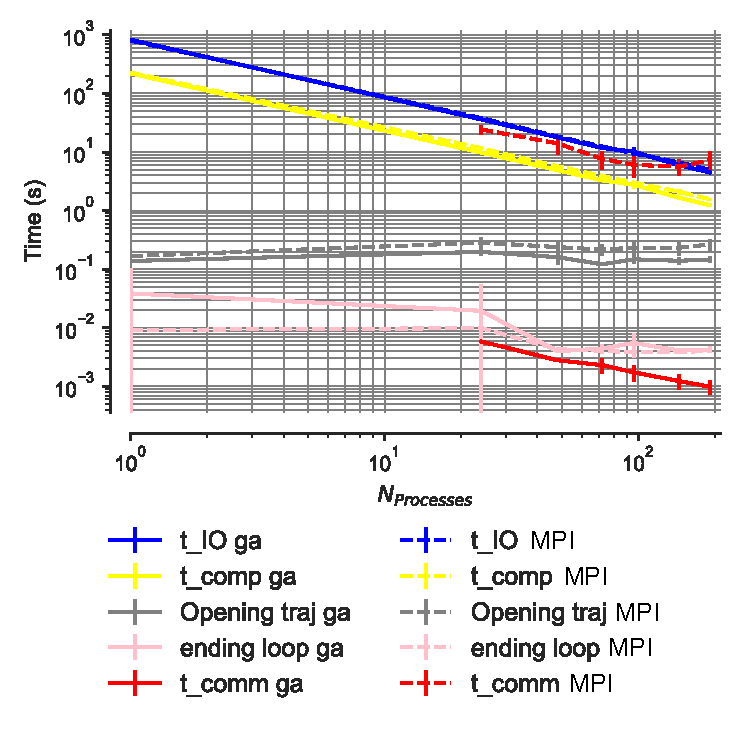
\includegraphics[width=\linewidth]{figures/Comparison_IO_compute_scaling_traj_splitting_edited.pdf}
    \captionsetup{format=hang}
    \caption{Scaling for different components}
    \label{fig:ScalingComputeIO-split}
  \end{subfigure}
  \hfill
  \begin{subfigure}{.3\textwidth}
    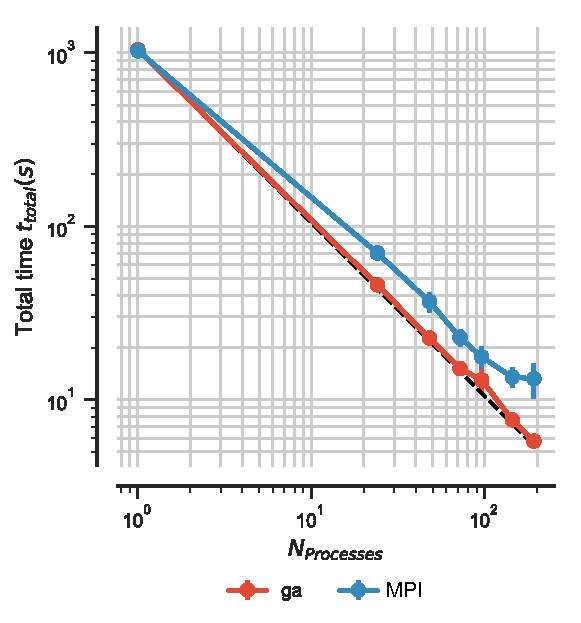
\includegraphics[width=\linewidth]{figures/Comparison_tot_time_traj_splitting_edited.pdf}
    \caption{Scaling total}
    \label{fig:MPIscaling-split}
  \end{subfigure}
  \hfill
  \begin{subfigure}{.3\textwidth}
    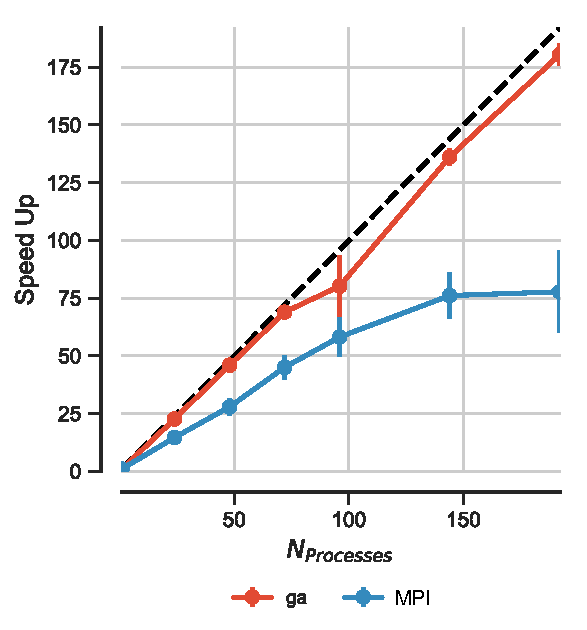
\includegraphics[width=\linewidth]{figures/Comparison_Speed_UP_traj_splitting_edited.pdf}
    \captionsetup{format=hang}
    \caption{Speed-up}
    \label{fig:MPIspeedup-split}
  \end{subfigure}
  \bigskip

  \begin{subfigure} {.45\textwidth}
    \includegraphics[width=\linewidth]{figures/split-BarPlot-rank-comparison_192_5.pdf}
    \captionsetup{format=hang}
    \caption{Time comparison on different parts of the calculations per MPI rank with MPI collective communications.}
    \label{fig:MPIranks-split}
  \end{subfigure}
  \hfill
  \begin{subfigure} {.5\textwidth}
    \includegraphics[width=\linewidth]{figures/split-ga-BarPlot-rank-comparison_192_5.pdf}
    \captionsetup{format=hang}
    \caption{Time comparison on different parts of the calculations per MPI rank using \package{Global Arrays}}
    \label{fig:MPIranks-split-ga}
\end{subfigure}
\caption{Comparison of the performance of the RMSD task on \emph{SDSC Comet} when the trajectories are split (\emph{subfiling}).
  The communication step used either MPI collective communications (``MPI'', with \texttt{MPI\_Gather()}) or  \package{Global Arrays} (``ga'', as described in Section~\protect\ref{Global-Array}).
  In the case of Global Arrays, all ranks updated the global RMSD array (\texttt{ga\_put()}) and rank 0 accessed the whole RMSD array through the global memory address (\texttt{ga\_get()}).
  Five repeats were performed to collect statistics.
  (a) Compute and I/O scaling versus number of processes.
  In serial, there is no communication and no data points are shown for $N=1$.
  (b) Total time scaling versus number of processes.
  (c) Speed-up.
  (a-c) The error bars show standard deviation with respect to the mean.
  (d-e) Compute \tcomp, read I/O \tIO, communication \tcomm, access to the whole global RMSD array by rank 0, $t_{\text{Access\_Global\_Array}}$, ending the for loop $t_{\text{end\_loop}}$, opening the trajectory $t_{\text{opening\_trajectory}}$, and overheads $t_{\text{overhead1}}$, $t_{\text{overhead2}}$ per MPI rank; see Table \ref{tab:notation} for the definitions.
}
\label{fig:MPIwithIO-split}
\end{figure}


The subfiling approach appeared promising but it required preprocessing of trajectory files and additional storage space for the segments.
We benchmarked the necessary time for splitting the trajectory in parallel using different number of MPI processes (Table~\ref{tab:timing-splitting}); in general the operation scaled well, with efficiencies $> 0.8$ although performance fluctuated, as seen for the case on six nodes where the efficiency dropped to $0.34$ for the run.
These preprocessing times were not included in the estimates because we focused on better understanding the principal causes of stragglers and we wanted to make the results directly comparable to the results of the previous sections.
Nevertheless, from an end user perspective, preprocessing of trajectories can be integrated in workflows (especially as the data in Table~\ref{tab:timing-splitting} indicated good scaling) and the preprocessing time can be quickly amortized if the trajectories are analyzed repeatedly.

\begin{table}[!htb]
  \centering
  \begin{tabular}{rrrrrr}
    \toprule
    \thead{$N_{\text{seg}}$} & \thead{$N_{\text{p}}$} & \thead{nodes}
    & \thead{time (s)} & \thead{$S$} & \thead{$E$}\\
    \midrule
    24 &  24 & 1 & 89.9 & 1.0 & 1.0\\
    48 &  48 & 2 & 46.8 & 1.9 & 0.96\\
    72 &  72 & 3 & 33.7 & 2.7 & 0.89\\
    96 &  96 & 4 & 25.1 & 3.6 & 0.89\\
    144 & 144 & 6 & 43.7 & 2.1 & 0.34\\
    192 & 192 & 8 & 13.5 & 6.7 & 0.83\\  
    \bottomrule
  \end{tabular}
  \caption[Time necessary for writing the trajectory segments]
  {The wall-clock time spent for writing $N_{\text{seg}}$ trajectory segments using $N_{\text{p}}$ processes using MPI on \emph{SDSC Comet}.
    One set of runs was performed for the timings.
    Scaling $S$ and efficiency $E$ are relative to the 1 node case (24 MPI processes).}
  \label{tab:timing-splitting}
\end{table}


Often trajectories from MD simulations on HPC machines are produced and kept in smaller files or segments that can be concatenated to form a full continuous trajectory file.
These trajectory segments could be used for the subfiling approach.
However, it might not be feasible to have exactly one segment per MPI rank, with all segments of equal size, which constitutes the ideal case for subfiling.
MDAnalysis can create virtual trajectories from separate trajectory segment files that appear to the user as a single trajectory.
In~\ref{sec:chainreader} we investigated if this so-called \emph{ChainReader} functionality could benefit from the subfiling approach.
We found some improvements in performance but discovered limitations in the design of the ChainReader (namely that all segment files are initially opened) that will have to be addressed before equivalent performance can be reached.
 
\subsubsection{MPI-based Parallel HDF5}
\label{HDF5}

In the HPC community, parallel I/O with MPI-IO is widely used in order to address I/O limitations.
We investigated MPI-based Parallel HDF5 to improve I/O scaling. 
We converted our XTC trajectory file into a simple custom HDF5 format so that we could test the performance of parallel I/O with the HDF5 file format.
The code for this file format conversion can be found in the GitHub repository.
The time it took to convert our XTC file with $2,512,200$ frames into HDF5 format was about 5,400~s on a local workstation with network file system (NFS).

\begin{figure}[!htb]
  \centering
  \begin{subfigure}{.49\textwidth}
    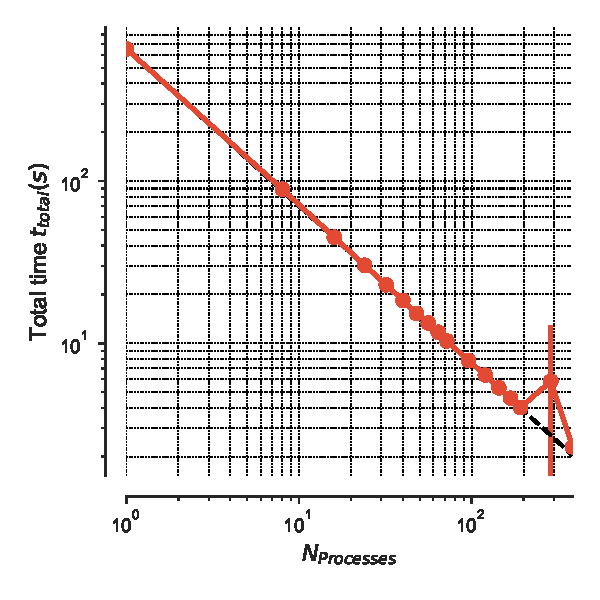
\includegraphics[width=\linewidth]{figures/hdf5-t_total.pdf}
    \caption{Scaling total}
    \label{fig:MPIscaling-hdf5}
  \end{subfigure}
  \hfill
  \begin{subfigure}{.49\textwidth}
    \includegraphics[width=\linewidth]{figures/hdf5-speed_up.pdf}
    \caption{Speed-up}
    \label{fig:MPIspeedup-hdf5}
  \end{subfigure}
  \bigskip

  \begin{subfigure}{.49\textwidth}
    \centering
    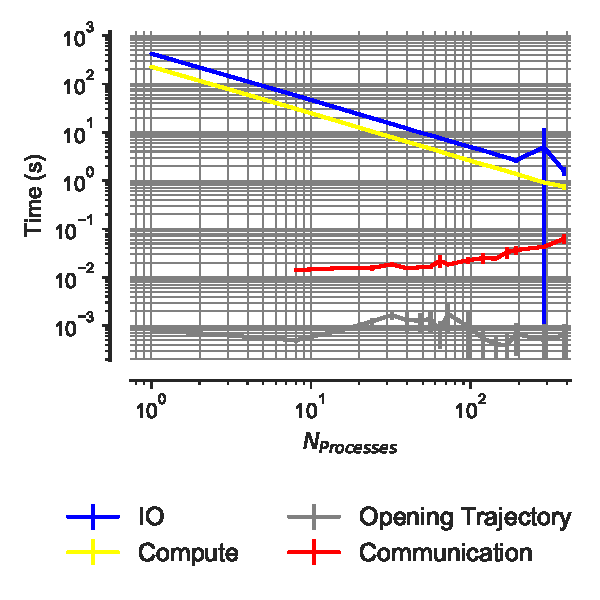
\includegraphics[width=\linewidth]{figures/hdf5-time_comp_IO_comparison.pdf}
    \captionsetup{format=hang}
    \caption{Scaling for different components}
    \label{fig:ScalingComputeIO-hdf5}
  \end{subfigure}
  \hfill
  \begin{subfigure} {.5\textwidth}
    \includegraphics[width=\linewidth]{figures/hdf5-BarPlot-rank-comparison_192_4.pdf}
    \captionsetup{format=hang}
    \caption{Time comparison on different parts of the calculations per MPI rank}
    \label{fig:MPIranks-hdf5}
  \end{subfigure}
  \caption{Performance of the RMSD task with MPI-based parallel HDF5 (MPI-IO) on \emph{SDSC Comet}.
    Data are read from the file system from a shared HDF5 file format instead of XTC format (independent I/O) and results are communicated back to rank 0. 
    Five repeats were performed to collect statistics.
    (a-c) The error bars show standard deviation with respect to the mean.
    In serial, there is no communication and no data points are shown for $N=1$ in (c).
    (d) Compute \tcomp, read I/O \tIO, communication \tcomm, ending the for loop $t_{\text{end\_loop}}$,
    opening the trajectory $t_{\text{opening\_trajectory}}$, and overheads $t_{\text{overhead1}}$, $t_{\text{overhead2}}$ per MPI rank; see Table \ref{tab:notation} for definitions.
    These are typical data from one run of the five repeats.
  }
  \label{fig:MPIwithIO-hdf5}
  %  I am reporting the slowest rank per timing, and that is averaged over all repeats.
\end{figure}

We ran our benchmark on up to 16 nodes (384 cores) on \emph{SDSC Comet} and we observed near ideal scaling behavior Figures~\ref{fig:MPIscaling-hdf5} and~\ref{fig:MPIspeedup-hdf5}) with parallel efficiencies above 0.8 on up to 8 nodes (Figure~\ref{fig:comparison_efficiency}) with no straggler tasks (Figure~\ref{fig:MPIranks-hdf5}).
The trajectory reading I/O (\tIO) was the dominant contribution, followed by compute (\tcomp), but because both contributions scaled well, overall scaling performance remained good, even for 384 cores.
We observed a low-performing outlier for 12 nodes (288 cores) with slower I/O than typical but did not further investigate.
Importantly, the trajectory opening cost remained negligible (in the millisecond range) and the cost for MPI communication also remained small (below 0.1 s, even for 16 nodes).
Overall, parallel MPI with HDF5 appeared to be a robust approach to obtain good scaling, even for I/O-bound tasks.


\subsection{Testing the Global Arrays Toolkit}
\label{Global-Array}

The \package{Global Arrays} (GA) toolkit \cite{GA} is a convenient layer to represent and access arrays across multiple MPI ranks and nodes.
Because of its convenience and possibly reduced communications overhead due to its use of shared memory on a physical node and MPI for inter-node communication (see Section~\ref{sec:methods-ga}) we wanted to compare parallel trajectory analysis with GA to the MPI-based implementation that was discussed in the previous sections.

\begin{figure}[!htb]
  \centering
  \begin{subfigure}{.49\textwidth}
    \includegraphics[width=\linewidth]{figures/RMSD-ga4py-t_total.pdf}
    \captionsetup{format=hang}
    \caption{Scaling total}
    \label{fig:MPIscaling-ga4py}
  \end{subfigure}
  \hfill
  \begin{subfigure}{.49\textwidth}
    \includegraphics[width=\linewidth]{figures/RMSD-ga4py-speed_up.pdf}
    \captionsetup{format=hang}
    \caption{Speed-up}
    \label{fig:MPIspeedup-ga4py}
  \end{subfigure}
  \bigskip

  \begin{subfigure}{.49\textwidth}
    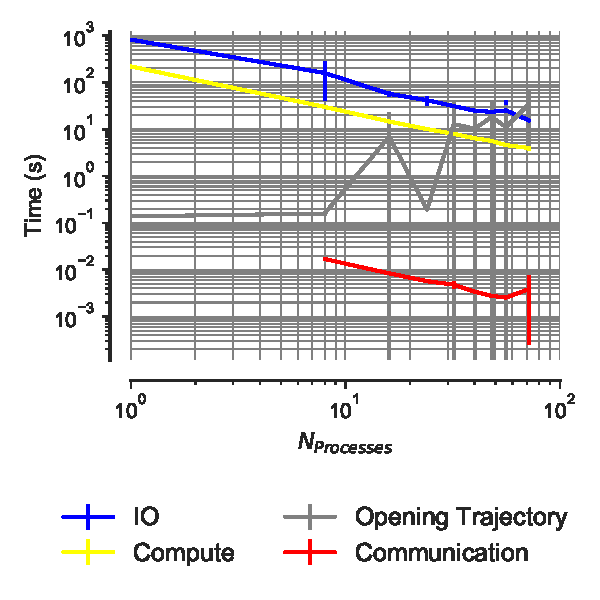
\includegraphics[width=\linewidth]{figures/RMSD-ga4py-time_IO_comparison.pdf}
    \captionsetup{format=hang}
    \caption{Scaling for different components}
    \label{fig:ScalingComputeIO-ga4py}
  \end{subfigure}
  \hfill
  \begin{subfigure} {.5\textwidth}
    \includegraphics[width=\linewidth]{figures/RMSD-ga4py-BarPlot-rank-comparison_72_1.pdf}
    \captionsetup{format=hang}
    \caption{Time comparison on different parts of the calculations per MPI rank}
    \label{fig:MPIranks-ga4py}
  \end{subfigure}
  \caption{Performance of the RMSD task using \package{Global Arrays} on \emph{SDSC Comet}.
    All ranks updated the global RMSD array (\texttt{ga\_put()}) and rank 0 accessed the whole RMSD array through the global memory address (\texttt{ga\_get()}).
    Five repeats were performed to collect statistics. (a-c) The error bars show standard deviation with respect to the mean. 
    In serial, there is no communication and not data points are shown for $N=1$ in (c).
    In (d), compute \tcomp, read I/O \tIO, communication \tcomm, access to the whole global array by rank 0, $t_{\text{Access\_Global\_Array}}$, ending the for loop $t_{\text{end\_loop}}$,
    opening the trajectory $t_{\text{opening\_trajectory}}$, and overheads $t_{\text{overhead1}}$, $t_{\text{overhead2}}$ per MPI rank are shown; see Table \ref{tab:notation} for definitions. 
    These are typical data from one run of the five repeats.
    MPI ranks 20 and 56 were stragglers.
  }
\label{fig:MPIwithIO-ga4py}
\end{figure}

With GA, one large RMSD array called the \emph{global array} was defined and each MPI rank updated its associated block in the global RMSD array using \texttt{ga\_put()} (Algorithm~\ref{alg:GA}).
At the end, when all the processes exited the \texttt{block\_rmsd()} function and updated their local block in the global array, rank 0  accessed the whole global array using \texttt{ga\_access()}.
In GA, the time for communication is $t_{\text{ga\_put()}}+t_{\text{ga\_access()}}$. 
We tested that the approach with GA (Algorithm~\ref{alg:GA}) gave the same results as the previously discussed approach with \texttt{MPI\_Gather()} (Algorithm~\ref{alg:RMSD}).


\paragraph{Shared file}
Using GA improved the strong scaling performance (Figures~\ref{fig:MPIscaling-ga4py} and~\ref{fig:MPIspeedup-ga4py}) by reducing the communication time.
Nevertheless, the remaining variation in the trajectory I/O part of the calculation and in particular the initial opening of the trajectory prevented ideal scaling (Figure~\ref{fig:ScalingComputeIO-ga4py}).
Stragglers were primarily due to the fact that all ranks had to open the same trajectory file at the beginning of the execution (Figure~\ref{fig:MPIranks-ga4py}).
In this case, these slow processes took about 50~s, which was slower than the mean execution time of all other ranks of 17~s. 
Trajectory opening was already problematic in the initial test (Figure~\ref{fig:ScalingComputeIO}), which was still dominated by the communication cost.
By substantially reducing communication cost, the simultaneous trajectory opening by multiple ranks emerged as the next dominant cause for stragglers.


\paragraph{Subfiling}
We tested subfiling (see Section~\ref{splitting-traj}) with GA to reduce the initial delay due to trajectory opening.
Under otherwise identical conditions as in the previous section we now observed near ideal scaling behavior with efficiencies above 0.9 (Figure~\ref{fig:MPIscaling-split} and~\ref{fig:MPIspeedup-split}) without any straggler tasks (Figure~\ref{fig:MPIranks-split-ga}).
Although the reason why in our case GA appeared to be more efficient than direct MPI-based communication remained unclear, these results showed that contention for file access clearly impacted performance.
By removing the contention, near ideal scaling could be achieved.


\subsection{Likely Causes of Stragglers}
\label{sec:likelycauses}

The data indicated that an increase in the duration of both MPI communication and trajectory file access lead to large variability in the run time of individual MPI processes and ultimately poor scaling performance beyond a single node.
A discussion of likely causes for stragglers begins with the observation that opening and reading a single trajectory file from multiple MPI processes appeared to be at the center of the problem. 

In MDAnalysis, individual trajectory frames are loaded into memory, which ensures that even systems with tens of millions of atoms can be efficiently analyzed on resources with moderate RAM sizes.
The test trajectory (file size 30 GB) had $2,512,200$ frames in total so each frame was about 0.011 MB in size.
With $\tIO \approx 0.3~\text{ms}$ per frame, the data were ingested at a rate of about $40$~MB/s for a single process.
For 24 MPI ranks (one \emph{SDSC Comet} node), the aggregated reading rate would have been about 1 GB/s, well within the available bandwidth of 56 Gb/s of the InfiniBand network interface that served the Lustre file system, but nevertheless sufficient to produce substantial constant network traffic.

Furthermore, in our study the default Lustre stripe size value was 1~MB, i.e., the amount of contiguous data stored on a single Lustre object storage target (OST).
Each I/O request read a single Lustre stripe but because the I/O size (0.011~MB) was smaller than the stripe size, many of these I/O requests were likely just accessing the same stripe on the same OST but nevertheless had to acquire a new reading lock for each request.
The reason for this behavior is related to ensuring POSIX consistency that relates to POSIX I/O API and POSIX I/O semantics, which can have adverse effects on scalability and performance.
Parallel file systems like Lustre implement sophisticated distributed locking mechanisms to ensure consistency.
For example, locking mechanisms ensures that a node can not read from a file or part of a file while it might be being modified by another node. 
In fact, when the application I/O is not designed in a way to avoid scenarios where multiple nodes are fighting over locks for overlapping extents, Lustre can suffer from scalability limitations~\cite{optimize_lustre}.
Continuously keeping metadata updated in order to have fully consistent reads and writes (POSIX metadata management), requires writing a new value for the file's last-accessed time (POSIX atime) every time a file is read, imposing a significant burden on parallel file system~\cite{POSIX2017}. 
It was observed that contention for the interconnect between OSTs and compute nodes due to MPI communication may lead to variable performance in I/O measurements~\cite{Mache:2005aa}.
Conversely, our data suggest that single-shared-file I/O on Lustre can negatively affect MPI communication as well, even at moderate numbers (tens to hundreds) of concurrent requests, similar to recent network simulations that predicted interference between MPI and I/O traffic~\cite{Brown:2018ab}.
This work indicated that MPI traffic (inter-process communication) can be affected by increasing I/O, and in particular, a few MPI processes were always delayed by one to two orders of magnitude more than the median time.
In summary, these observations in the context of the work by \citet{Brown:2018ab} suggest that our observed stragglers with large variance in the communication step might be due to interference of MPI communications with the I/O requests on the same network.

